\chapter{Graph-Datenbanken im praktischen Einsatz: OLAP}
\section{PostgreSQL: OLAP}
\subsection{Benchmark}
Mit der Standardinstallation von PostgreSQL wird auch pgbench mitinstalliert. Bei pgbench handelt es sich um ein einfaches Tool zur Durchführung von Benchmark-Tests. Bei einem Benchmark-Test wird eine Menge von \ac{SQL}-Statements beliebig oft wiederholt, dabei können auch mehrere parallele Sessions geöffnet werden. Beim durchführen des Tests berechnet pgbench die Anzahl der Transaktionen pro Sekunde.
\subsubsection{Verwendung von pgbench}
pgbench wird über die Kommandozeile gestartet. Dabei können eine Reihe von Parametern übergeben werden, mit denen das Verhalten von pgbench gesteuert werden kann.
\begin{itemize}
	\item -c clients  \\
	Über das Flag -c wird die Anzahl der Clients bzw. die Anzahl der gleichzeitigen Datenbankverbindungen festgelegt. Wenn hier nichts angegeben ist wird nur ein Client verewendet.
	\item -t transactions \\
	Über das Flag -t wird festgelegt wieviele Transaktionen jeder Client durchführt. Die Anzahl aller Transaktionen ergibt sich durch das Produkt von Clients und Transactions.
\end{itemize}
\subsubsection{Antwortzeiten ohne Indices}
\begin{figure}[H]
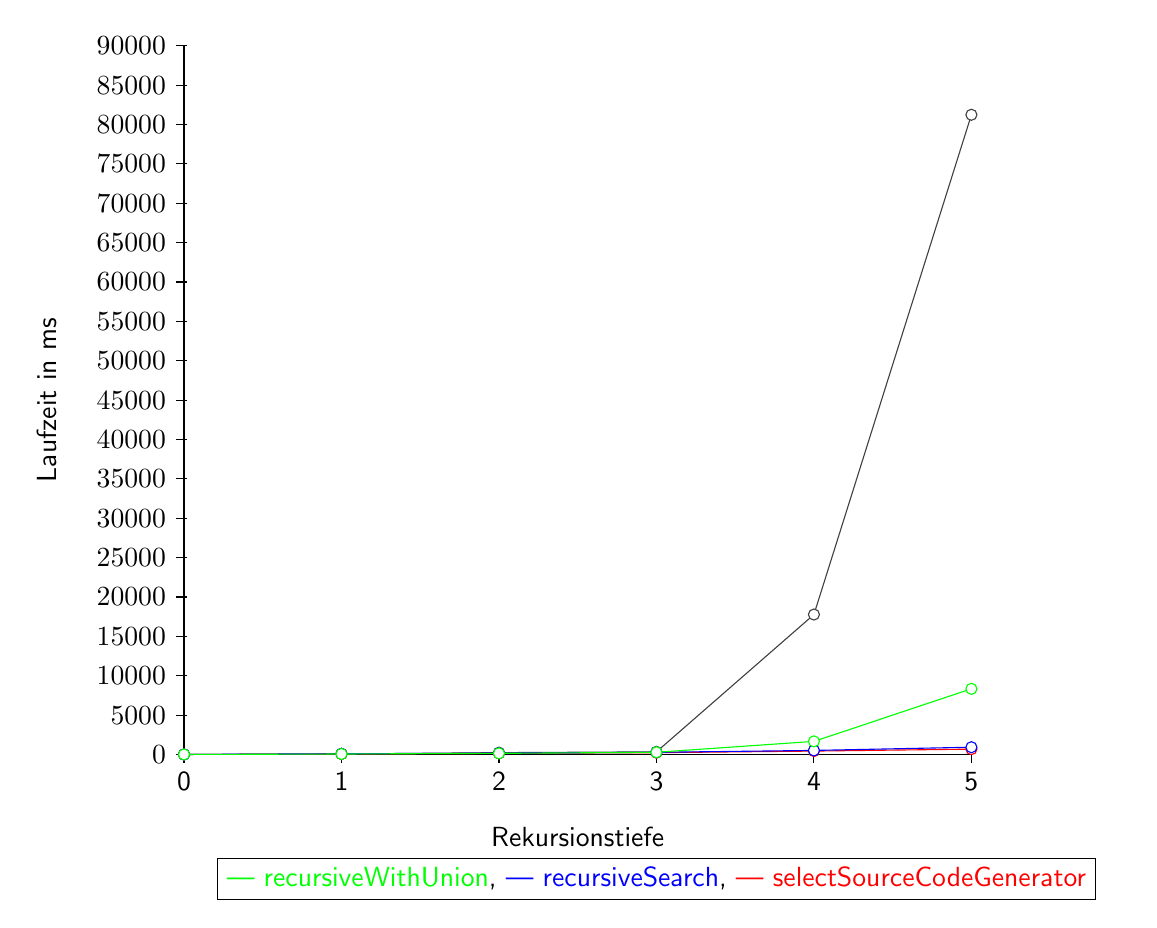
\begin{tikzpicture}[y=.5cm, x=2cm,font=\sffamily]
%axis
\draw (0,0) -- coordinate (x axis mid) (5,0);
\draw (0,0) -- coordinate (y axis mid) (0,18);
    	%ticks
\foreach \x in {0,...,5}
\draw (\x,1pt) -- (\x,-3pt)
node[anchor=north] {\x};
	\foreach \y/\ytext in {
	0/0,
	1/5000,
	2/10000,
	3/15000,
	4/20000,
	5/25000,
	6/30000,
	7/35000,
	8/40000,
	9/45000,
	10/50000,
	11/55000,
	12/60000,
	13/65000,
	14/70000,
	15/75000,
	16/80000,
	17/85000,
	18/90000
}
\draw (1pt,\y) -- (-3pt,\y) node[anchor=east] {$\ytext$}; 
%labels      
\node[below=0.8cm] at (x axis mid) {Rekursionstiefe};
\node[rotate=90, above=1.5cm] at (y axis mid) {Laufzeit in ms};
%plots
\draw[darkgray] plot[ mark=*, mark options={fill=white}] 
coordinates{(0, 0)
	(1, 61.065/5000)
	(2,231.850/5000)
	(3,333.011/5000)
	(4,3.5545)%17772.456/5000)
	(5,16.2483)%81241.284/5000
};

\draw[red] plot[ mark=*, mark options={fill=white}] 
coordinates{(0, 0)
			(1, 63.636/5000)
			(2,139.225/5000)
			(3,229.997/5000)
			(4,432.297/5000)
			(5,677.420/5000)
		};
\draw[blue] plot[ mark=*, mark options={fill=white}] 
coordinates{(0, 0)
	(1, 89.858/5000)
	(2,168.822/5000)
	(3,273.452/5000)
	(4,513.038/5000)
	(5,921.228/5000)
};
\draw[green] plot[ mark=*, mark options={fill=white}] 
coordinates{(0, 0)
	(1, 59.275/5000)
	(2,143.367/5000)
	(3,277.766/5000)
	(4,1664.168/5000)
	(5,8335.513/5000)
};
\draw[draw=none] (0,0) -- (6,0) node[draw, midway, yshift=-4.5em] {\textcolor{green}{--- recursiveWithUnion},
	\textcolor{blue}{--- recursiveSearch}, 
	\textcolor{red}{--- selectSourceCodeGenerator}};
\end{tikzpicture}
	\caption{ public\_epinions}
\end{figure}


% Please add the following required packages to your document preamble:
% \usepackage{multirow}
\begin{table}[H]
	\begin{tabular}{l|l|l|l|l|l|}
		\cline{2-6}
		& \multicolumn{5}{|l|}{Laufzeit in MS}                                                                                                                                                  \\ \hline
		\multicolumn{1}{|l|}{\multirow{2}{2cm}{Rerkusions-tiefe}} & \multicolumn{2}{|l|}{\multirow{2}{3cm}{selectSource CodeGenerator}} & \multirow{2}{2.8cm}{recursiveSearch} & \multirow{2}{2.5cm}{recursive WithUnion} & \multirow{2}{2.5cm}{selectInner JoinGenerator} \\
		\multicolumn{1}{|l|}{}
		& \multicolumn{2}{|l|}{}                                           &                                  &                                     &                                           \\ \hline
	\multicolumn{1}{|l|}{1}               & \multicolumn{2}{l|}{63.636}                                     & 89.858                           & 59.275                              & 61.065                                    \\ \hline
	\multicolumn{1}{|l|}{2}               & \multicolumn{2}{l|}{139.225}                                    & 168.822                          & 143.367                             & 231.850                                   \\ \hline
	\multicolumn{1}{|l|}{3}               & \multicolumn{2}{l|}{229.997}                                    & 273.452                          & 277.766                             & 333.011                                   \\ \hline
	\multicolumn{1}{|l|}{4}               & \multicolumn{2}{l|}{432.297}                                    & 513.038                          & 1664.168                            & 17772.456                                 \\ \hline
	\multicolumn{1}{|l|}{5}               & \multicolumn{2}{l|}{677.420}                                    & 921.228                          & 8335.513                            & 81241.284                                 \\ \hline
	
	\end{tabular}
\end{table}
\begin{figure}[H]
	
	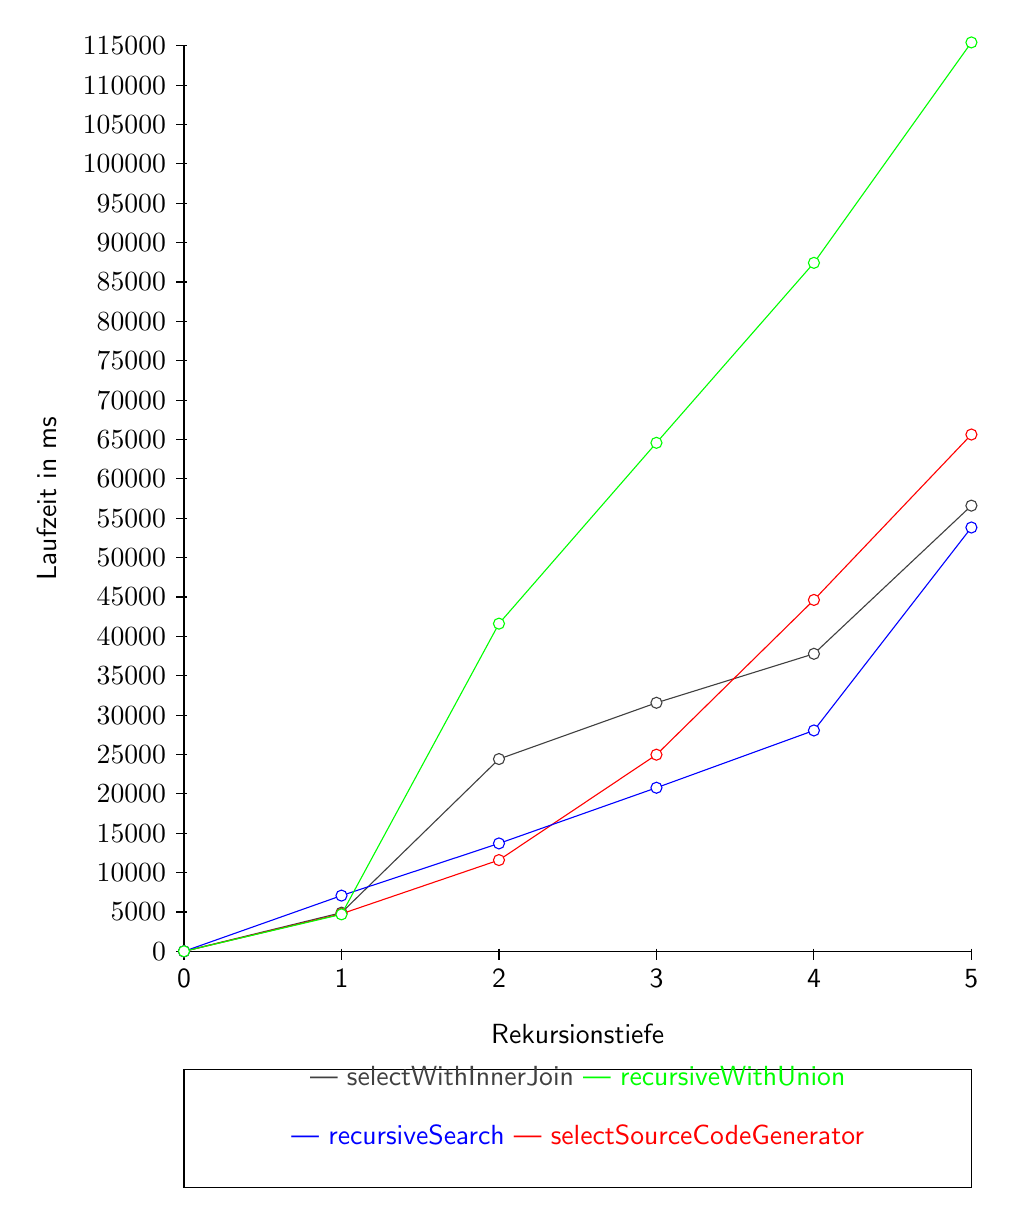
\begin{tikzpicture}[y=.5cm, x=2cm,font=\sffamily]
	%axis
	\draw (0,0) -- coordinate (x axis mid) (5,0);
	\draw (0,0) -- coordinate (y axis mid) (0,23);
	%ticks
	\foreach \x in {0,...,5}
	\draw (\x,1pt) -- (\x,-3pt)
	node[anchor=north] {\x};
	\foreach \y/\ytext in {
		0/0,
		1/5000,
		2/10000,
		3/15000,
		4/20000,
		5/25000,
		6/30000,
		7/35000,
		8/40000,
		9/45000,
		10/50000,
		11/55000,
		12/60000,
		13/65000,
		14/70000,
		15/75000,
		16/80000,
		17/85000,
		18/90000,
		19/95000,
		20/100000,
		21/105000,
		22/110000,
		23/115000
	}
	\draw (1pt,\y) -- (-3pt,\y) node[anchor=east] {$\ytext$};
	%labels      
	\node[below=0.8cm] at (x axis mid) {Rekursionstiefe};
	\node[rotate=90, above=1.5cm] at (y axis mid) {Laufzeit in ms};
	%plots
	\draw[darkgray] plot[mark=*, mark options={fill=white}] 
	coordinates{(0, 0)
		(1, 0.9819)%4909.862/5000)
		(2,	4.8836)%24417.787/5000)
		(3, 6.3127)%31563.339/5000)
		(4, 7.5570)%37785.200/5000)
		(5,	11.3202)%56601.185/5000)
	};
	\draw[red] plot[mark=*, mark options={fill=white}] 
	coordinates{(0, 0)
		(1, 4761.733/5000)
		(2,	11589.219/5000)
		(3, 4.9944)	%=24971/5000
		(4, 8.9252) %=44625,935÷5000
		(5,	13.1265944)%=65632,972÷5000
	};
\draw[blue] plot[mark=*, mark options={fill=white}] 
coordinates{(0, 0)
	(1, 1.4151)%7075.399/5000)
	(2,	2.7405)%13702.381/5000)
	(3, 4.1548)%20773.827/5000)
	(4, 5.6098)%28048.866/5000)
	(5,	10.7651)%53825.401/5000)
};
\draw[green] plot[mark=*, mark options={fill=white}] 
coordinates{(0, 0)
	(1, 0.939)%4695.466/5000)
	(2,	8.323)%41616.216/5000)
	(3, 12.916)%64577.873/5000)
	(4, 17.487)%87434.075/5000)	
	(5,	23.086)%115432.071/5000)	
};
	\draw (0,-3) -- (5,-3) 
(0,-3) -- (0,-6)
(0,-6) -- (5,-6)
(5,-3) -- (5,-6);
\draw[draw=none] (0,0) -- (5,0) 
node[draw=none, midway, yshift=-4.5em]
{
	\textcolor{darkgray}{--- selectWithInnerJoin}
	\textcolor{green}{--- recursiveWithUnion} 
	
};
\draw[draw=none] (0,-3) -- (5,0) 
node[draw=none, midway, yshift=-4.5em]
{
	\textcolor{blue}{--- recursiveSearch} 
	\textcolor{red}{--- selectSourceCodeGenerator}
};
	\end{tikzpicture}
	\caption{ public\_livejournal}
\end{figure}
\begin{table}[H]
	\begin{tabular}{l|l|l|l|l|l|}
		\cline{2-6}
		& \multicolumn{5}{|l|}{Laufzeit in MS}                                                                                                                                                  \\ \hline
		\multicolumn{1}{|l|}{\multirow{2}{2cm}{Rerkusions-tiefe}} & \multicolumn{2}{|l|}{\multirow{2}{3cm}{selectSource CodeGenerator}} & \multirow{2}{2.8cm}{recursiveSearch} & \multirow{2}{2.5cm}{recursive WithUnion} & \multirow{2}{2.5cm}{selectInner JoinGenerator} \\
		\multicolumn{1}{|l|}{}
		& \multicolumn{2}{|l|}{}                                           &                                  &                                     &                                           \\ \hline
		\multicolumn{1}{|l|}{1}                                 & \multicolumn{2}{l|}{4761.733}                                    & 7075.399                                              & 4695.466                                                  & 4909.862                                                        \\ \hline
		\multicolumn{1}{|l|}{2}                                 & \multicolumn{2}{l|}{11589.219}                                   & 13702.381                                             & 41616.216                                                 & 24417.787                                                       \\ \hline
		\multicolumn{1}{|l|}{3}                                 & \multicolumn{2}{l|}{24971}                                       & 20773.831                                             & 64577.873                                                 & 31563.339                                                       \\ \hline
		\multicolumn{1}{|l|}{4}                                 & \multicolumn{2}{l|}{44625.935}                                   & 28048.866                                             & 87434.075                                                 & 37785.200                                                       \\ \hline
		\multicolumn{1}{|l|}{5}                                 & \multicolumn{2}{l|}{65632.972}                                   & 53825.401                                             & 115432.071                                                & 56601.185                                                       \\ \hline
		
	\end{tabular}
\end{table}


\begin{figure}[H]
	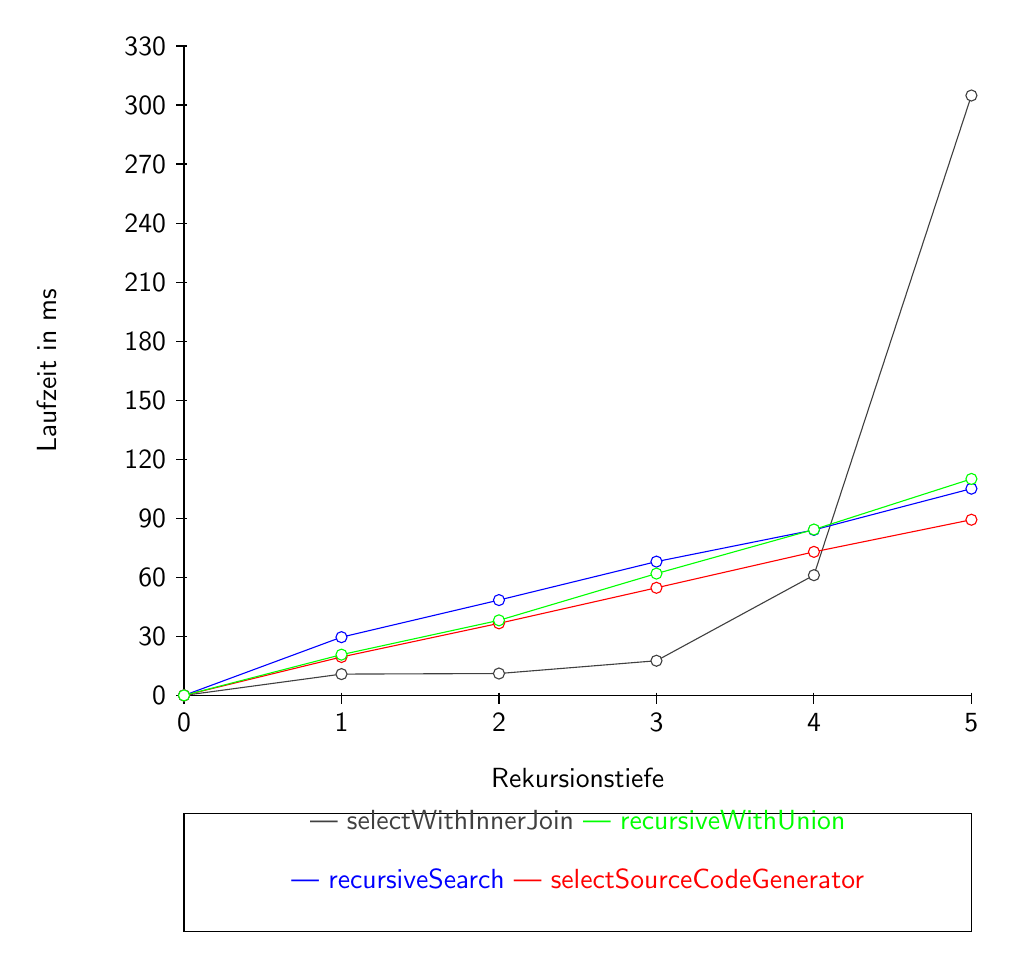
\begin{tikzpicture}[y=.025cm, x=2cm,font=\sffamily]
	%axis
	\draw (0,0) -- coordinate (x axis mid) (5,0);
	\draw (0,0) -- coordinate (y axis mid) (0,330);
	%ticks
	\foreach \x in {0,...,5}
	\draw (\x,1pt) -- (\x,-3pt)
	node[anchor=north] {\x};
	\foreach \y in {0,30,...,330}
	\draw (1pt,\y) -- (-3pt,\y)
	node[anchor=east] {\y}; 
	%labels      
	\node[below=0.8cm] at (x axis mid) {Rekursionstiefe};
	\node[rotate=90, above=1.5cm] at (y axis mid) {Laufzeit in ms};
	%plots
	\draw[darkgray] plot[ mark=*, mark options={fill=white}] 
	coordinates{(0, 0)
		(1, 10.825)
		(2, 11.119)
		(3, 17.613)
		(4, 61.089)
		(5, 304.821)
	};
	
	\draw[blue] plot[ mark=*, mark options={fill=white}] 
	coordinates{(0, 0)
		(1, 29.595)
		(2,48.442)
		(3,67.989)
		(4,84.084)
		(5,105.049)
	};
	\draw[red] plot[ mark=*, mark options={fill=white}] 
	coordinates{(0, 0)
		(1, 19.528)
		(2,36.613)
		(3,54.681)
		(4,72.934)
		(5,89.262)
	};
	\draw[green] plot[ mark=*, mark options={fill=white}] 
	coordinates{(0, 0)
		(1, 20.716)
		(2,38.137)
		(3,61.904)
		(4,84.295)
		(5,110.000)
	};

	\draw (0,-60) -- (5,-60) 
		  (0,-60) -- (0,-120)
          (0,-120) -- (5,-120)
          (5,-60) -- (5,-120);
\draw[draw=none] (0,0) -- (5,0) 
node[draw=none, midway, yshift=-4.5em]
{
	\textcolor{darkgray}{--- selectWithInnerJoin}
	\textcolor{green}{--- recursiveWithUnion} 
	
};
\draw[draw=none] (0,-60) -- (5,0) 
node[draw=none, midway, yshift=-4.5em]
{
	\textcolor{blue}{--- recursiveSearch} 
	\textcolor{red}{--- selectSourceCodeGenerator}
};
	\end{tikzpicture}
	\caption{ public\_facebook}
\end{figure}

\begin{figure}[H]
	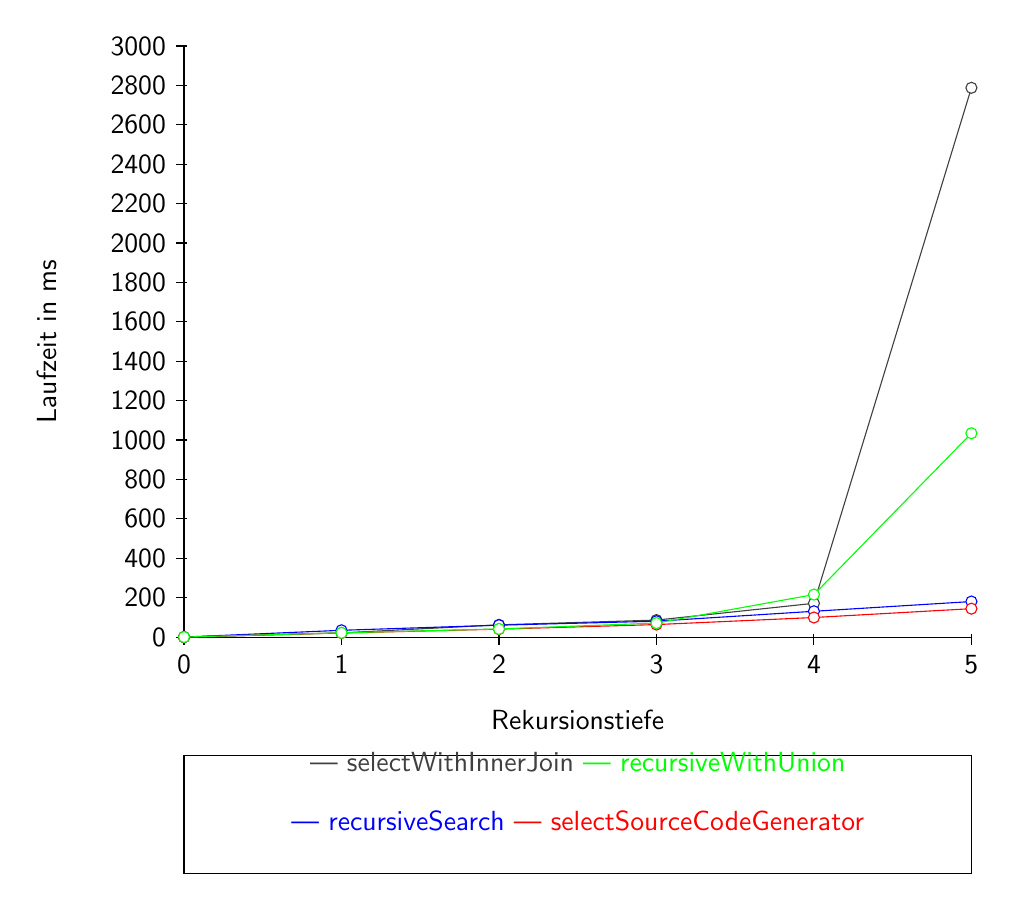
\begin{tikzpicture}[y=.0025cm, x=2cm,font=\sffamily]
	%axis
	\draw (0,0) -- coordinate (x axis mid) (5,0);
	\draw (0,0) -- coordinate (y axis mid) (0,3000);
	%ticks
	\foreach \x in {0,...,5}
	\draw (\x,1pt) -- (\x,-3pt)
	node[anchor=north] {\x};
	\foreach \y in {0,200,...,3000}
	\draw (1pt,\y) -- (-3pt,\y)
	node[anchor=east] {\y}; 
	%labels      
	\node[below=0.8cm] at (x axis mid) {Rekursionstiefe};
	\node[rotate=90, above=1.5cm] at (y axis mid) {Laufzeit in ms};
	%plots
	\draw[darkgray] plot[ mark=*, mark options={fill=white}] 
	coordinates{(0, 0)
		(1, 21.182)
		(2, 62.066)
		(3, 86.128)
		(4, 171.283)
		(5, 2787.659)
	};
	
	\draw[blue] plot[ mark=*, mark options={fill=white}] 
	coordinates{(0, 0)
		(1, 34.365)
		(2, 60.394)
		(3, 80.454)
		(4, 130.866)
		(5, 180.301)
	};
	\draw[red] plot[ mark=*, mark options={fill=white}] 
	coordinates{(0, 0)
		(1, 20.774)
		(2, 40.090)
		(3, 63.405)
		(4, 99.210)
		(5, 144.089)
	};
	\draw[green] plot[ mark=*, mark options={fill=white}] 
	coordinates{(0, 0)
		(1, 21.490)
		(2, 41.234)
		(3, 70.961)
		(4, 215.687)
		(5,1034.360)
	};
	
	\draw (0,-600) -- (5,-600) 
	(0,-600) -- (0,-1200)
	(0,-1200) -- (5,-1200)
	(5,-600) -- (5,-1200);
	\draw[draw=none] (0,0) -- (5,0) 
	node[draw=none, midway, yshift=-4.5em]
	{
		\textcolor{darkgray}{--- selectWithInnerJoin}
		\textcolor{green}{--- recursiveWithUnion} 
		
	};
	\draw[draw=none] (0,-600) -- (5,0) 
	node[draw=none, midway, yshift=-4.5em]
	{
		\textcolor{blue}{--- recursiveSearch} 
		\textcolor{red}{--- selectSourceCodeGenerator}
	};
	\end{tikzpicture}
	\caption{ public\_wiki\_vote}
\end{figure}

\begin{figure}[H]
	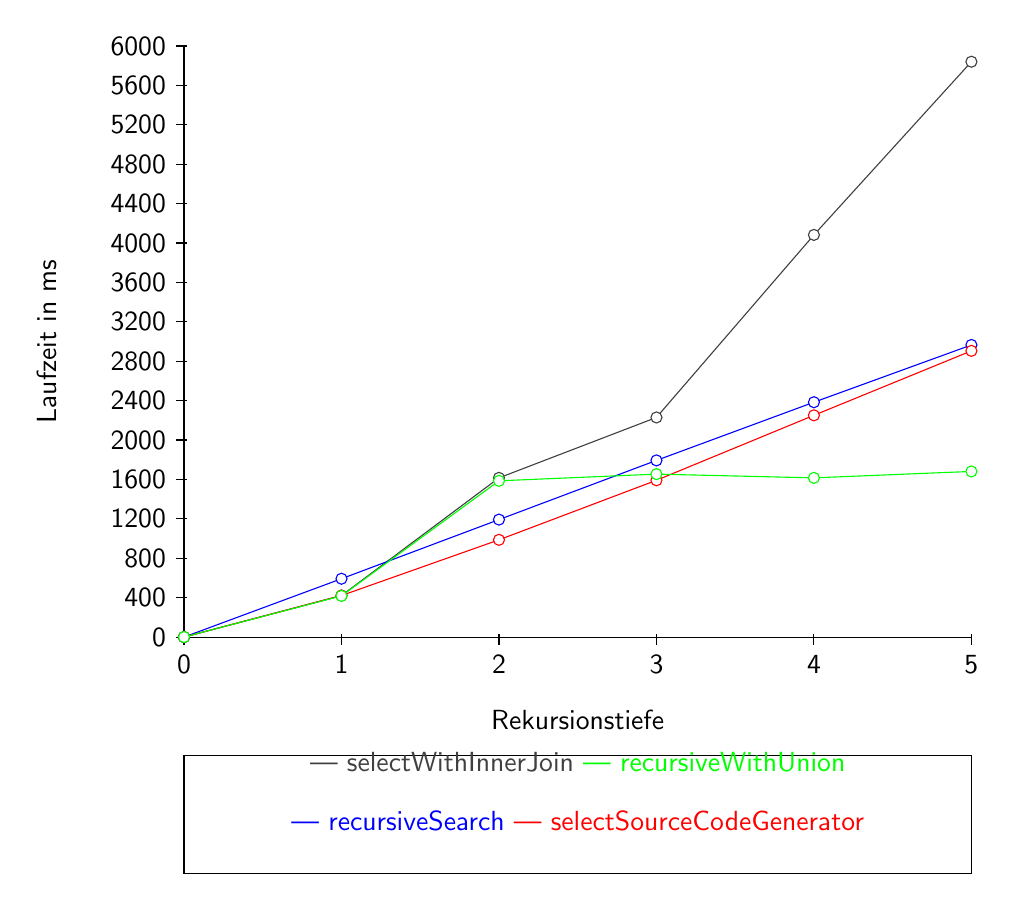
\begin{tikzpicture}[y=.00125cm, x=2cm,font=\sffamily]
	%axis
	\draw (0,0) -- coordinate (x axis mid) (5,0);
	\draw (0,0) -- coordinate (y axis mid) (0,6000);
	%ticks
	\foreach \x in {0,...,5}
	\draw (\x,1pt) -- (\x,-3pt)
	node[anchor=north] {\x};
	\foreach \y in {0,400,...,6000}
	\draw (1pt,\y) -- (-3pt,\y)
	node[anchor=east] {\y}; 
	%labels      
	\node[below=0.8cm] at (x axis mid) {Rekursionstiefe};
	\node[rotate=90, above=1.5cm] at (y axis mid) {Laufzeit in ms};
	%plots
	\draw[darkgray] plot[ mark=*, mark options={fill=white}] 
	coordinates{(0, 0)
		(1, 421.124)
		(2, 1615.843)
		(3, 2229.214)
		(4, 4082.179)
		(5, 5839.987)
	};
	
	\draw[blue] plot[ mark=*, mark options={fill=white}] 
	coordinates{(0, 0)
		(1, 592.063)
		(2, 1192.278)
		(3, 1793.281)
		(4, 2383.885)
		(5, 2964.950)
	};
	\draw[red] plot[ mark=*, mark options={fill=white}] 
	coordinates{(0, 0)
		(1, 421.464)
		(2, 986.995)
		(3, 1591.391)
		(4, 2250.832)
		(5, 2905.167)
	};
	\draw[green] plot[ mark=*, mark options={fill=white}] 
	coordinates{(0, 0)
		(1, 418.105)
		(2, 1585.836)
		(3, 1654.011)
		(4, 1615.986)
		(5, 1681.231)
	};
	
	\draw (0,-1200) -- (5,-1200) 
	(0,-1200) -- (0,-2400)
	(0,-2400) -- (5,-2400)
	(5,-1200) -- (5,-2400);
	\draw[draw=none] (0,0) -- (5,0) 
	node[draw=none, midway, yshift=-4.5em]
	{
		\textcolor{darkgray}{--- selectWithInnerJoin}
		\textcolor{green}{--- recursiveWithUnion} 
		
	};
	\draw[draw=none] (0,-1200) -- (5,0) 
	node[draw=none, midway, yshift=-4.5em]
	{
		\textcolor{blue}{--- recursiveSearch} 
		\textcolor{red}{--- selectSourceCodeGenerator}
	};
	\end{tikzpicture}
	\caption{ public\_youtube}
\end{figure}

\subsubsection{Antwortzeiten mit Indices}


\begin{figure}[H]
	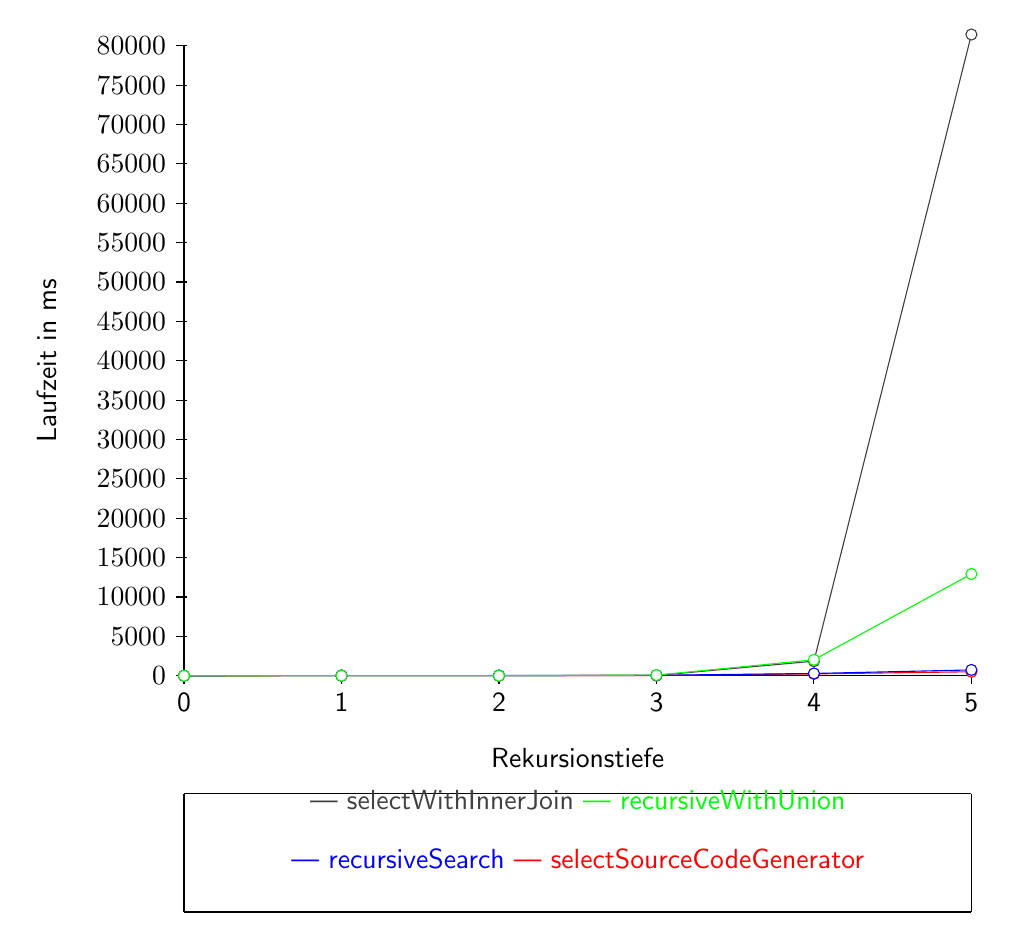
\begin{tikzpicture}[y=.5cm, x=2cm,font=\sffamily]
	%axis
	\draw (0,0) -- coordinate (x axis mid) (5,0);
	\draw (0,0) -- coordinate (y axis mid) (0,16);
	%ticks
	\foreach \x in {0,...,5}
	\draw (\x,1pt) -- (\x,-3pt)
	node[anchor=north] {\x};
	\foreach \y/\ytext in {
		0/0,
		1/5000,
		2/10000,
		3/15000,
		4/20000,
		5/25000,
		6/30000,
		7/35000,
		8/40000,
		9/45000,
		10/50000,
		11/55000,
		12/60000,
		13/65000,
		14/70000,
		15/75000,
		16/80000
	}
		\draw (1pt,\y) -- (-3pt,\y) node[anchor=east] {$\ytext$}; 
	%labels      
	\node[below=0.8cm] at (x axis mid) {Rekursionstiefe};
	\node[rotate=90, above=1.5cm] at (y axis mid) {Laufzeit in ms};
	%plots
	\draw[darkgray] plot[ mark=*, mark options={fill=white}] 
	coordinates{(0, 0)
		(1, 10.596/5000)
		(2, 10.739/5000)
		(3, 41.171/5000)
		(4, 0.3696)%1898.726/5000
		(5, 16.2872)%81436.561/5000
	};
	
	\draw[red] plot[ mark=*, mark options={fill=white}] 
	coordinates{(0, 0)
		(1, 8.231/5000)
		(2, 9.290/5000)
		(3, 36.244/5000)
		(4, 235.146/5000)
		(5, 504.793/5000)
	};
	\draw[blue] plot[ mark=*, mark options={fill=white}] 
	coordinates{(0, 0)
		(1, 18.999/5000)
		(2, 23.549/5000)
		(3, 54.953/5000)
		(4, 287.319/5000)
		(5, 737.300/5000)
	};
	\draw[green] plot[ mark=*, mark options={fill=white}] 
	coordinates{(0, 0)
		(1, 8.855/5000)
		(2, 10.304/5000)
		(3, 78.303/5000)
		(4, 2024.069/5000)
		(5, 12920.747/5000)
	};
	\draw (0,-3) -- (5,-3) 
(0,-3) -- (0,-6)
(0,-6) -- (5,-6)
(5,-3) -- (5,-6);
\draw[draw=none] (0,0) -- (5,0) 
node[draw=none, midway, yshift=-4.5em]
{
	\textcolor{darkgray}{--- selectWithInnerJoin}
	\textcolor{green}{--- recursiveWithUnion} 
	
};
\draw[draw=none] (0,-3) -- (5,0) 
node[draw=none, midway, yshift=-4.5em]
{
	\textcolor{blue}{--- recursiveSearch} 
	\textcolor{red}{--- selectSourceCodeGenerator}
};
	\end{tikzpicture}
	\caption{ public\_epinions}
\end{figure}


\begin{table}[H]
	\centering
	\begin{tabular}{l|l|l|l|}
		\cline{2-4}
		& \multicolumn{3}{l|}{Laufzeit in MS} \\ \hline
		\multicolumn{1}{|l|}{Rerkusionstiefe} & selectSourceCodeGenerator  & recursiveSearch  & recursiveWithUnion    \\ \hline
		\multicolumn{1}{|l|}{1}               & 8.231           & 	18.999  & 8.855    \\ \hline
		\multicolumn{1}{|l|}{2}               & 9.290          & 	23.549 & 10.304   \\ \hline
		\multicolumn{1}{|l|}{3}               & 36.244          &  54.953   &  78.303   \\ \hline
		\multicolumn{1}{|l|}{4}               & 235.146          &  287.319     & 2024.069     \\ \hline
		\multicolumn{1}{|l|}{5}               & 504.793          &  737.300   & 12920.747     \\ \hline
	\end{tabular}
\end{table}

\begin{figure}[H]
	
	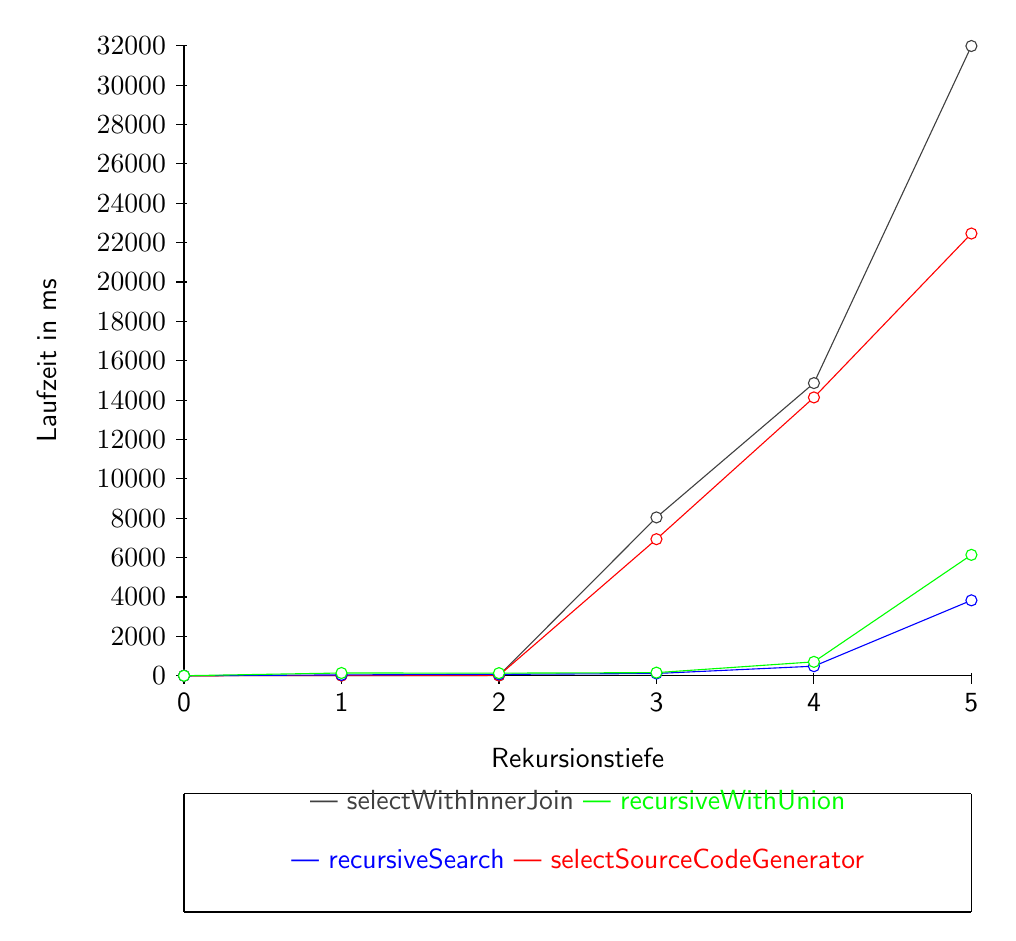
\begin{tikzpicture}[y=.5cm, x=2cm,font=\sffamily]
	%axis
	\draw (0,0) -- coordinate (x axis mid) (5,0);
	\draw (0,0) -- coordinate (y axis mid) (0,16);
	%ticks
	\foreach \x in {0,...,5}
	\draw (\x,1pt) -- (\x,-3pt)
	node[anchor=north] {\x};
	\foreach \y/\ytext in {
		0/0,
		1/2000,
		2/4000,
		3/6000,
		4/8000,
		5/10000,
		6/12000,
		7/14000,
		8/16000,
		9/18000,
		10/20000,
		11/22000,
		12/24000,
		13/26000,
		14/28000,
		15/30000,
		16/32000,
	}
	\draw (1pt,\y) -- (-3pt,\y) node[anchor=east] {$\ytext$};
	%labels      
	\node[below=0.8cm] at (x axis mid) {Rekursionstiefe};
	\node[rotate=90, above=1.5cm] at (y axis mid) {Laufzeit in ms};
	%plots
	
	\draw[darkgray] plot[mark=*, mark options={fill=white}] 
	coordinates{(0, 0)
		(1, 9.165/2000)
		(2,	11.862/2000)
		(3, 8042.794/2000)
		(4, 14865.814/2000)
		(5,	 15.995)%31990.436/2000)
	};	
	\draw[red] plot[mark=*, mark options={fill=white}] 
	coordinates{(0, 0)
		(1, 0.004)%8.672/2000
		(2,	15.240/2000)
		(3, 6936.935/2000)
		(4, 14137.544/2000)%
		(5,	11.232)%22464.363/2000	
	};
	\draw[blue] plot[mark=*, mark options={fill=white}] 
	coordinates{(0, 0)
		(1, 42.010/2000)
		(2,	69.129/2000)
		(3, 114.466/2000)
		(4, 484.914/2000)
		(5,	3830.355/2000)
	};
	\draw[green] plot[mark=*, mark options={fill=white}] 
	coordinates{(0, 0)
		(1, 139.294/2000)
		(2,	131.623/2000)
		(3, 157.707/2000)
		(4, 705.293/2000)
		(5, 6140.824/2000)
	};
	\draw (0,-3) -- (5,-3) 
(0,-3) -- (0,-6)
(0,-6) -- (5,-6)
(5,-3) -- (5,-6);
\draw[draw=none] (0,0) -- (5,0) 
node[draw=none, midway, yshift=-4.5em]
{
	\textcolor{darkgray}{--- selectWithInnerJoin}
	\textcolor{green}{--- recursiveWithUnion} 
	
};
\draw[draw=none] (0,-3) -- (5,0) 
node[draw=none, midway, yshift=-4.5em]
{
	\textcolor{blue}{--- recursiveSearch} 
	\textcolor{red}{--- selectSourceCodeGenerator}
};
	\end{tikzpicture}
	\caption{ public\_livejournal}
\end{figure}

\begin{figure}[H]
	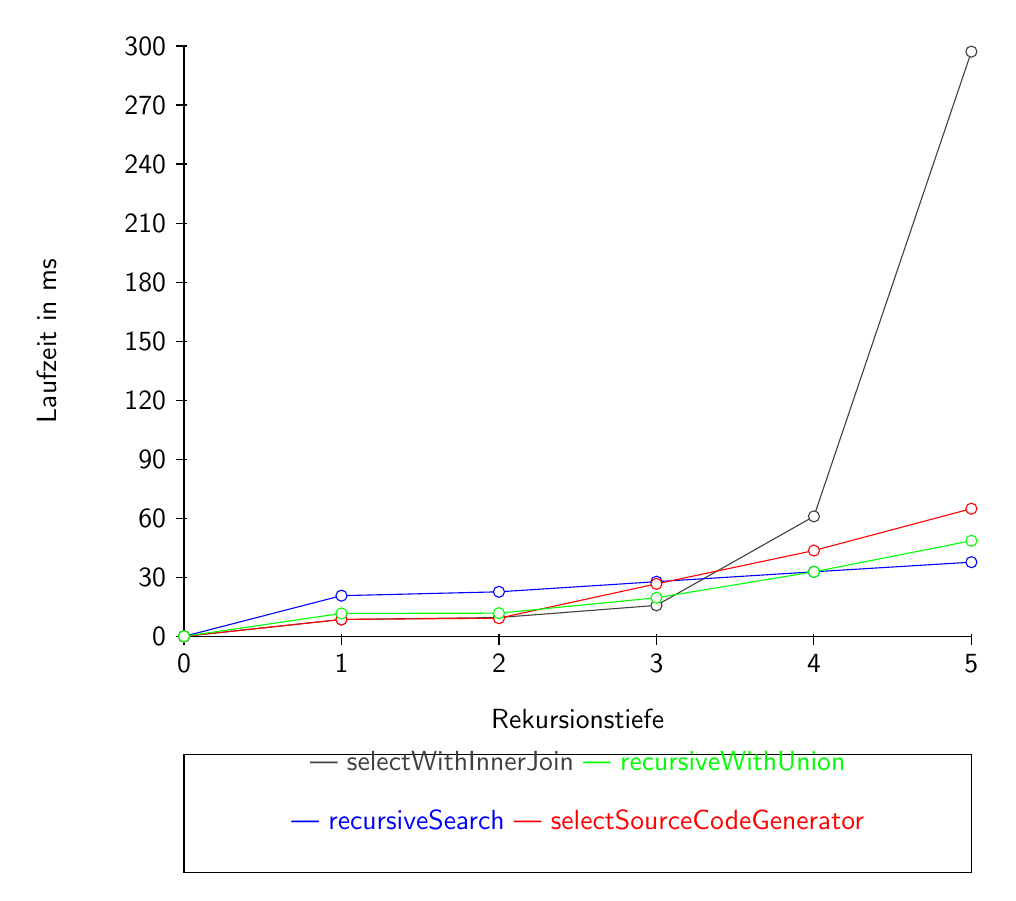
\begin{tikzpicture}[y=.025cm, x=2cm,font=\sffamily]
	%axis
	\draw (0,0) -- coordinate (x axis mid) (5,0);
	\draw (0,0) -- coordinate (y axis mid) (0,300);
	%ticks
	\foreach \x in {0,...,5}
	\draw (\x,1pt) -- (\x,-3pt)
	node[anchor=north] {\x};
	\foreach \y in {0,30,...,300}
	\draw (1pt,\y) -- (-3pt,\y)
	node[anchor=east] {\y}; 
	%labels      
	\node[below=0.8cm] at (x axis mid) {Rekursionstiefe};
	\node[rotate=90, above=1.5cm] at (y axis mid) {Laufzeit in ms};
	%plots
	\draw[darkgray] plot[ mark=*, mark options={fill=white}] 
	coordinates{(0, 0)
		(1, 8.585)
		(2, 9.565)
		(3, 15.738)
		(4, 60.976)
		(5, 297.115)
	};
	
	\draw[blue] plot[ mark=*, mark options={fill=white}] 
	coordinates{(0, 0)
		(1, 20.674)
		(2, 22.639)
		(3, 27.788)
		(4, 32.804)
		(5, 37.706)
	};
	\draw[red] plot[ mark=*, mark options={fill=white}] 
	coordinates{(0, 0)
		(1, 8.594)
		(2, 9.239)
		(3, 26.683)
		(4, 43.610)
		(5, 64.882)
	};
	\draw[green] plot[ mark=*, mark options={fill=white}] 
	coordinates{(0, 0)
		(1, 11.672)
		(2, 11.787)
		(3, 19.625)
		(4, 32.817)
		(5, 48.580)
	};
	
	\draw (0,-60) -- (5,-60) 
	(0,-60) -- (0,-120)
	(0,-120) -- (5,-120)
	(5,-60) -- (5,-120);
	\draw[draw=none] (0,0) -- (5,0) 
	node[draw=none, midway, yshift=-4.5em]
	{
		\textcolor{darkgray}{--- selectWithInnerJoin}
		\textcolor{green}{--- recursiveWithUnion} 
		
	};
	\draw[draw=none] (0,-60) -- (5,0) 
	node[draw=none, midway, yshift=-4.5em]
	{
		\textcolor{blue}{--- recursiveSearch} 
		\textcolor{red}{--- selectSourceCodeGenerator}
	};
	\end{tikzpicture}
	\caption{ public\_facebook}
\end{figure}

\begin{figure}[H]
	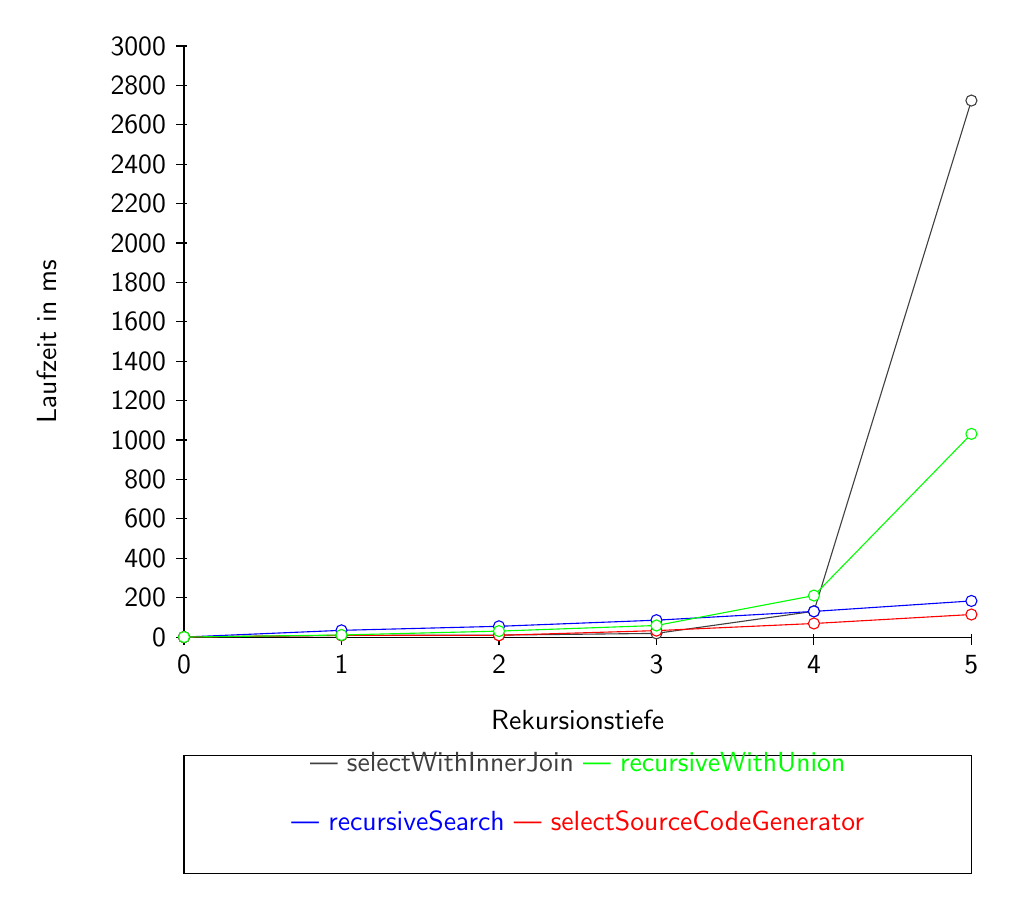
\begin{tikzpicture}[y=.0025cm, x=2cm,font=\sffamily]
	%axis
	\draw (0,0) -- coordinate (x axis mid) (5,0);
	\draw (0,0) -- coordinate (y axis mid) (0,3000);
	%ticks
	\foreach \x in {0,...,5}
	\draw (\x,1pt) -- (\x,-3pt)
	node[anchor=north] {\x};
	\foreach \y in {0,200,...,3000}
	\draw (1pt,\y) -- (-3pt,\y)
	node[anchor=east] {\y}; 
	%labels      
	\node[below=0.8cm] at (x axis mid) {Rekursionstiefe};
	\node[rotate=90, above=1.5cm] at (y axis mid) {Laufzeit in ms};
	%plots
	\draw[darkgray] plot[ mark=*, mark options={fill=white}] 
	coordinates{(0, 0)
		(1, 8.481)
		(2, 9.903)
		(3, 18.657)
		(4, 130.842)
		(5, 2722.908)
	};
	
	\draw[blue] plot[ mark=*, mark options={fill=white}] 
	coordinates{(0, 0)
		(1, 34.144)
		(2, 54.617)
		(3, 85.721)
		(4, 130.150)
		(5, 183.301)
	};
	\draw[red] plot[ mark=*, mark options={fill=white}] 
	coordinates{(0, 0)
		(1, 8.716)
		(2, 8.868)
		(3, 32.682)
		(4, 68.856)
		(5, 114.462)
	};
	\draw[green] plot[ mark=*, mark options={fill=white}] 
	coordinates{(0, 0)
		(1, 10.474)
		(2, 30.212)
		(3, 58.762)
		(4, 210.655)
		(5, 1031.234)
	};
	
	\draw (0,-600) -- (5,-600) 
	(0,-600) -- (0,-1200)
	(0,-1200) -- (5,-1200)
	(5,-600) -- (5,-1200);
	\draw[draw=none] (0,0) -- (5,0) 
	node[draw=none, midway, yshift=-4.5em]
	{
		\textcolor{darkgray}{--- selectWithInnerJoin}
		\textcolor{green}{--- recursiveWithUnion} 
		
	};
	\draw[draw=none] (0,-600) -- (5,0) 
	node[draw=none, midway, yshift=-4.5em]
	{
		\textcolor{blue}{--- recursiveSearch} 
		\textcolor{red}{--- selectSourceCodeGenerator}
	};
	\end{tikzpicture}
	\caption{ public\_wiki\_vote}
\end{figure}

\begin{figure}[H]
	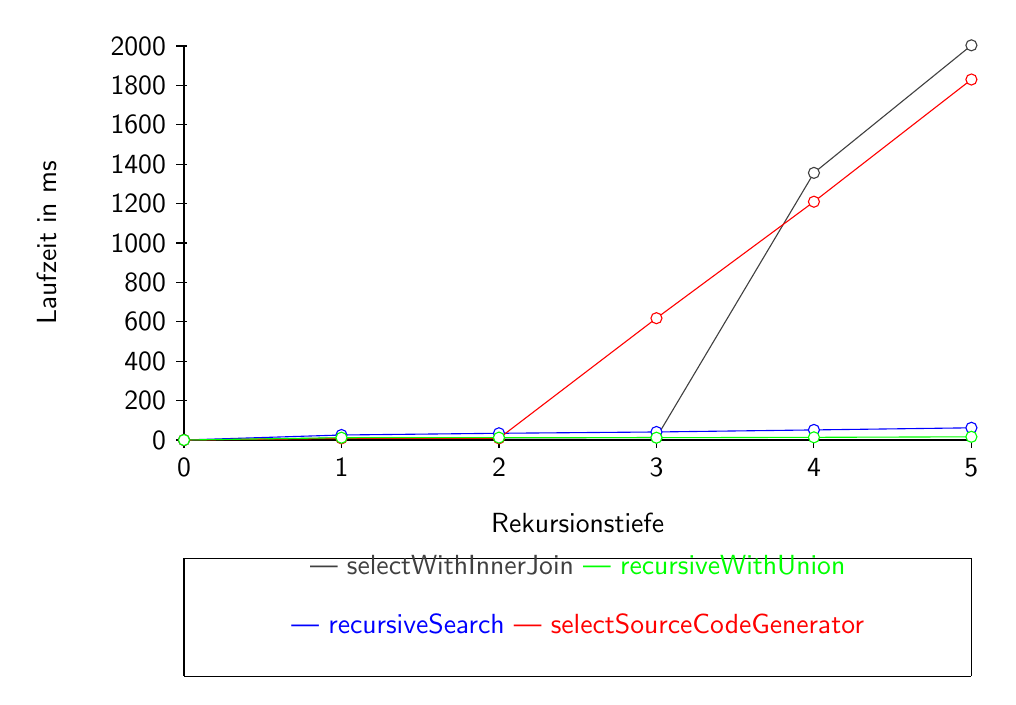
\begin{tikzpicture}[y=.0025cm, x=2cm,font=\sffamily]
	%axis
	\draw (0,0) -- coordinate (x axis mid) (5,0);
	\draw (0,0) -- coordinate (y axis mid) (0,2000);
	%ticks
	\foreach \x in {0,...,5}
	\draw (\x,1pt) -- (\x,-3pt)
	node[anchor=north] {\x};
	\foreach \y in {0,200,...,2000}
	\draw (1pt,\y) -- (-3pt,\y)
	node[anchor=east] {\y}; 
	%labels      
	\node[below=0.8cm] at (x axis mid) {Rekursionstiefe};
	\node[rotate=90, above=1.5cm] at (y axis mid) {Laufzeit in ms};
	%plots
	\draw[darkgray] plot[ mark=*, mark options={fill=white}] 
	coordinates{(0, 0)
		(1, 10.213)
		(2, 10.587)
		(3, 12.858)
		(4, 1355.866)
		(5, 2003.275)
	};
	
	\draw[blue] plot[ mark=*, mark options={fill=white}] 
	coordinates{(0, 0)
		(1, 25.508)
		(2, 34.273)
		(3, 40.852)
		(4, 51.285)
		(5, 62.037)
	};
	\draw[red] plot[ mark=*, mark options={fill=white}] 
	coordinates{(0, 0)
		(1, 8.370)
		(2, 8.528)
		(3, 618.336)
		(4, 1209.513)
		(5, 1829.757)
	};
	\draw[green] plot[ mark=*, mark options={fill=white}] 
	coordinates{(0, 0)
		(1, 11.801)
		(2, 12.265)
		(3, 11.832)
		(4, 13.644)
		(5, 16.362)
	};
	
	\draw (0,-600) -- (5,-600) 
	(0,-600) -- (0,-1200)
	(0,-1200) -- (5,-1200)
	(5,-600) -- (5,-1200);
	\draw[draw=none] (0,0) -- (5,0) 
	node[draw=none, midway, yshift=-4.5em]
	{
		\textcolor{darkgray}{--- selectWithInnerJoin}
		\textcolor{green}{--- recursiveWithUnion} 
		
	};
	\draw[draw=none] (0,-600) -- (5,0) 
	node[draw=none, midway, yshift=-4.5em]
	{
		\textcolor{blue}{--- recursiveSearch} 
		\textcolor{red}{--- selectSourceCodeGenerator}
	};
	\end{tikzpicture}
	\caption{ public\_youtube}
\end{figure}


\subsection{Antwortzeiten mit partitionierten Tabellen und Indices}

\begin{figure}[H]
	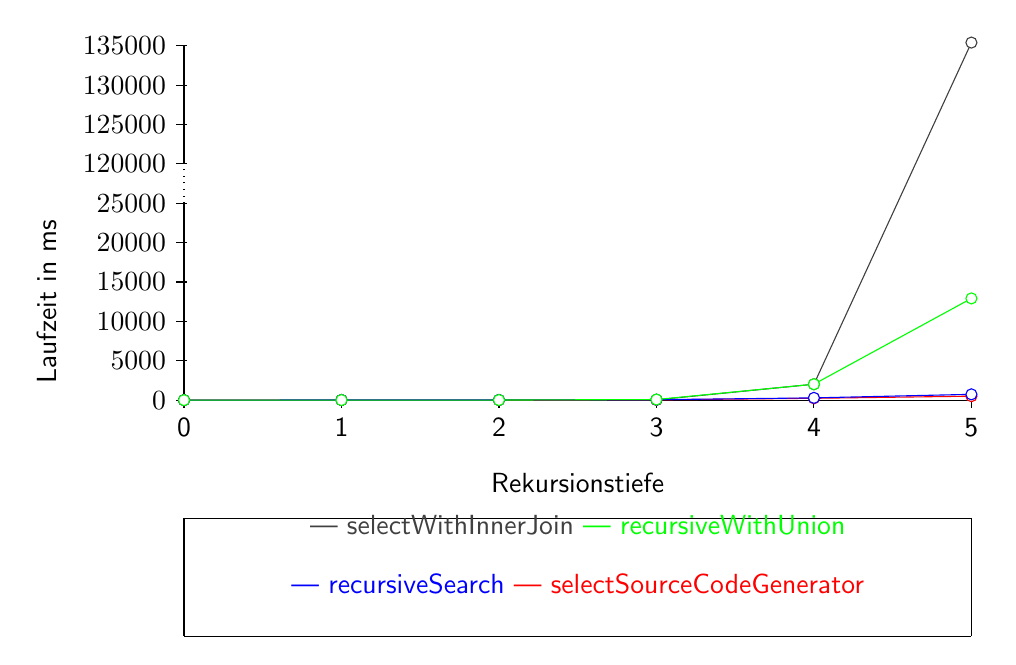
\begin{tikzpicture}[y=.5cm, x=2cm,font=\sffamily]
	%axis
	\draw (0,0) -- coordinate (x axis mid) (5,0);
	\draw (0,0) -- coordinate (y axis mid) (0,5);
	\draw[dotted] (0,5) -- (0,6);
	\draw (0,6) -- (0,9);
	%ticks
	\foreach \x in {0,...,5}
	\draw (\x,1pt) -- (\x,-3pt)
	node[anchor=north] {\x};
		\foreach \y/\ytext in {
		0/0,
		1/5000,
		2/10000,
		3/15000,
		4/20000,
		5/25000,
		6/120000,
		7/125000,
		8/130000,
		9/135000
	}
	\draw (1pt,\y) -- (-3pt,\y) node[anchor=east] {$\ytext$};
	%labels      
	\node[below=0.8cm] at (x axis mid) {Rekursionstiefe};
	\node[rotate=90, above=1.5cm] at (y axis mid) {Laufzeit in ms};
	%plots
	\draw[darkgray] plot[ mark=*, mark options={fill=white}] 
	coordinates{(0, 0)
		(1, 0.002)%8.846/5000)
		(2, 0.002)%9.924/5000)
		(3, 43.439/5000)
		(4, 2021.028/5000)
		(5, 9.082)%136242.608/15000)
	};
	
	\draw[red] plot[ mark=*, mark options={fill=white}] 
	coordinates{(0, 0)
		(1, 0.002)%8.231/5000)
		(2, 0.002)%9.290/5000)
		(3, 36.244/5000)
		(4, 235.146/5000)
		(5, 504.793/5000)
	};
	\draw[blue] plot[ mark=*, mark options={fill=white}] 
	coordinates{(0, 0)
		(1, 18.999/5000)
		(2, 23.549/5000)
		(3, 54.953/5000)
		(4, 287.319/5000)
		(5, 737.300/5000)
	};
	\draw[green] plot[ mark=*, mark options={fill=white}] 
	coordinates{(0, 0)
		(1, 8.855/5000)
		(2, 10.304/5000)
		(3, 78.303/5000)
		(4,2024.069/5000)
		(5,12920.747/5000)
	};
\draw (0,-3) -- (5,-3) 
(0,-3) -- (0,-6)
(0,-6) -- (5,-6)
(5,-3) -- (5,-6);
\draw[draw=none] (0,0) -- (5,0) 
node[draw=none, midway, yshift=-4.5em]
{
	\textcolor{darkgray}{--- selectWithInnerJoin}
	\textcolor{green}{--- recursiveWithUnion} 
	
};
\draw[draw=none] (0,-3) -- (5,0) 
node[draw=none, midway, yshift=-4.5em]
{
	\textcolor{blue}{--- recursiveSearch} 
	\textcolor{red}{--- selectSourceCodeGenerator}
};
	\end{tikzpicture}
	\caption{ public\_epinions}
\end{figure}



\begin{figure}[H]
	
	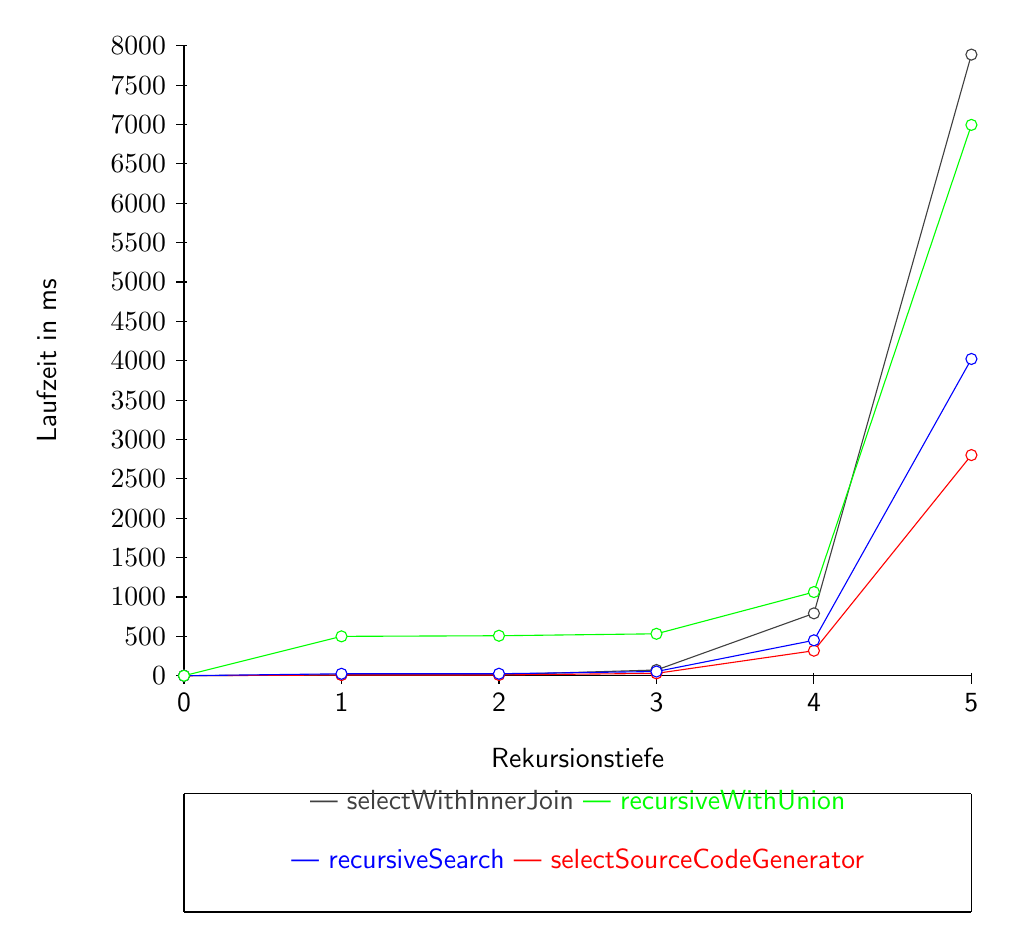
\begin{tikzpicture}[y=.5cm, x=2cm,font=\sffamily]
	%axis
	\draw (0,0) -- coordinate (x axis mid) (5,0);
	\draw (0,0) -- coordinate (y axis mid) (0,16);
	%ticks
	\foreach \x in {0,...,5}
	\draw (\x,1pt) -- (\x,-3pt)
	node[anchor=north] {\x};
	\foreach \y/\ytext in {
		0/0,
		1/500,
		2/1000,
		3/1500,
		4/2000,
		5/2500,
		6/3000,
		7/3500,
		8/4000,
		9/4500,
		10/5000,
		11/5500,
		12/6000,
		13/6500,
		14/7000,
		15/7500,
		16/8000
	}
	\draw (1pt,\y) -- (-3pt,\y) node[anchor=east] {$\ytext$};
	%labels      
	\node[below=0.8cm] at (x axis mid) {Rekursionstiefe};
	\node[rotate=90, above=1.5cm] at (y axis mid) {Laufzeit in ms};
	%plots
	%InnerJoin
	\draw[darkgray] plot[mark=*, mark options={fill=white}] 
	coordinates{(0, 0)
		(1, 11.849/500)
		(2,	13.616/500)
		(3, 72.842/500)
		(4, 792.107/500)
		(5,	7888.135/500)
	};
	%SelectGenerator
	\draw[red] plot[mark=*, mark options={fill=white}] 
	coordinates{(0, 0)
		(1, 0.018)%8.945/500
		(2,	9.875/500)
		(3, 29.855/500)
		(4, 317.921/500)%
		(5,	2802.370/500)	
	};
	%RecursiveSearch
	\draw[blue] plot[mark=*, mark options={fill=white}] 
	coordinates{(0, 0)
		(1, 24.721/500)
		(2,	25.354/500)
		(3, 53.544/500)
		(4, 449.968/500)
		(5,	4022.937/500)
	};
	%SelectWithUnion
	\draw[green] plot[mark=*, mark options={fill=white}] 
	coordinates{(0, 0)
		(1, 500.063/500)
		(2,	507.950/500)
		(3, 532.557/500)
		(4, 1062.957/500)
		(5, 6995.607/500)
	};
	
	\draw (0,-3) -- (5,-3) 
		  (0,-3) -- (0,-6)
		  (0,-6) -- (5,-6)
		  (5,-3) -- (5,-6);
	\draw[draw=none] (0,0) -- (5,0) 
	node[draw=none, midway, yshift=-4.5em]
	 {
	 	\textcolor{darkgray}{--- selectWithInnerJoin}
	 	\textcolor{green}{--- recursiveWithUnion} 
	
	};
	\draw[draw=none] (0,-3) -- (5,0) 
	node[draw=none, midway, yshift=-4.5em]
	{
		\textcolor{blue}{--- recursiveSearch} 
		\textcolor{red}{--- selectSourceCodeGenerator}
	};

	\end{tikzpicture}
	\caption{ public\_livejournal}
\end{figure}

\begin{figure}[H]
	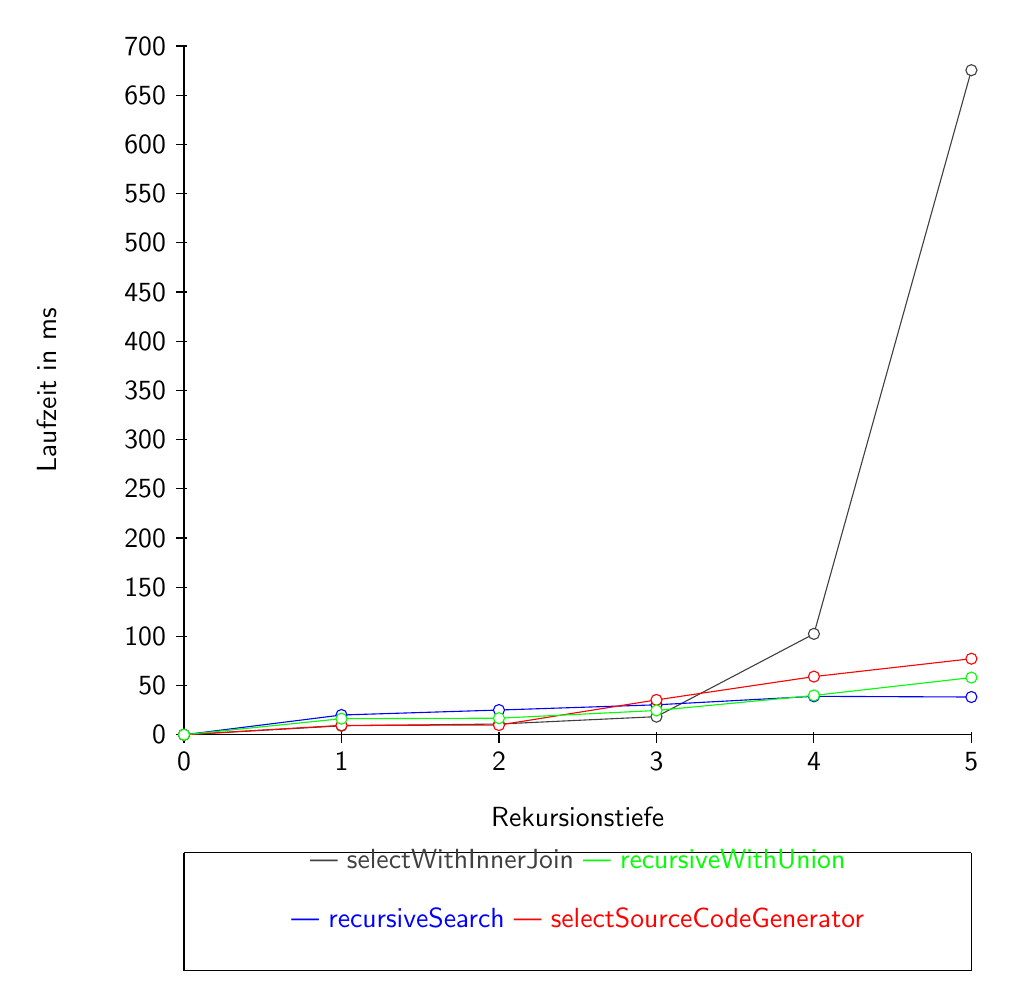
\begin{tikzpicture}[y=.0125cm, x=2cm,font=\sffamily]
	%axis
	\draw (0,0) -- coordinate (x axis mid) (5,0);
	\draw (0,0) -- coordinate (y axis mid) (0,700);
	%ticks
	\foreach \x in {0,...,5}
	\draw (\x,1pt) -- (\x,-3pt)
	node[anchor=north] {\x};
	\foreach \y in {0,50,...,700}
	\draw (1pt,\y) -- (-3pt,\y)
	node[anchor=east] {\y}; 
	%labels      
	\node[below=0.8cm] at (x axis mid) {Rekursionstiefe};
	\node[rotate=90, above=1.5cm] at (y axis mid) {Laufzeit in ms};
	%plots
	\draw[darkgray] plot[ mark=*, mark options={fill=white}] 
	coordinates{(0, 0)
		(1, 9.097)
		(2, 10.898)
		(3, 18.393)
		(4, 102.515)
		(5, 675.363)
	};
	
	\draw[blue] plot[ mark=*, mark options={fill=white}] 
	coordinates{(0, 0)
		(1, 20.057)
		(2, 25.119)
		(3, 30.430)
		(4, 39.050)
		(5, 38.354)
	};
	\draw[red] plot[ mark=*, mark options={fill=white}] 
	coordinates{(0, 0)
		(1, 9.550)
		(2, 9.838)
		(3, 35.418)
		(4, 59.112)
		(5, 77.279)
	};
	\draw[green] plot[ mark=*, mark options={fill=white}] 
	coordinates{(0, 0)
		(1, 16.339)
		(2, 16.807)
		(3, 24.669)
		(4, 39.953)
		(5, 58.086)
	};
	
	\draw (0,-120) -- (5,-120) 
	(0,-120) -- (0,-240)
	(0,-240) -- (5,-240)
	(5,-120) -- (5,-240);
	\draw[draw=none] (0,0) -- (5,0) 
	node[draw=none, midway, yshift=-4.5em]
	{
		\textcolor{darkgray}{--- selectWithInnerJoin}
		\textcolor{green}{--- recursiveWithUnion} 
		
	};
	\draw[draw=none] (0,-120) -- (5,0) 
	node[draw=none, midway, yshift=-4.5em]
	{
		\textcolor{blue}{--- recursiveSearch} 
		\textcolor{red}{--- selectSourceCodeGenerator}
	};
	\end{tikzpicture}
	\caption{ public\_facebook}
\end{figure}

\begin{figure}[H]
	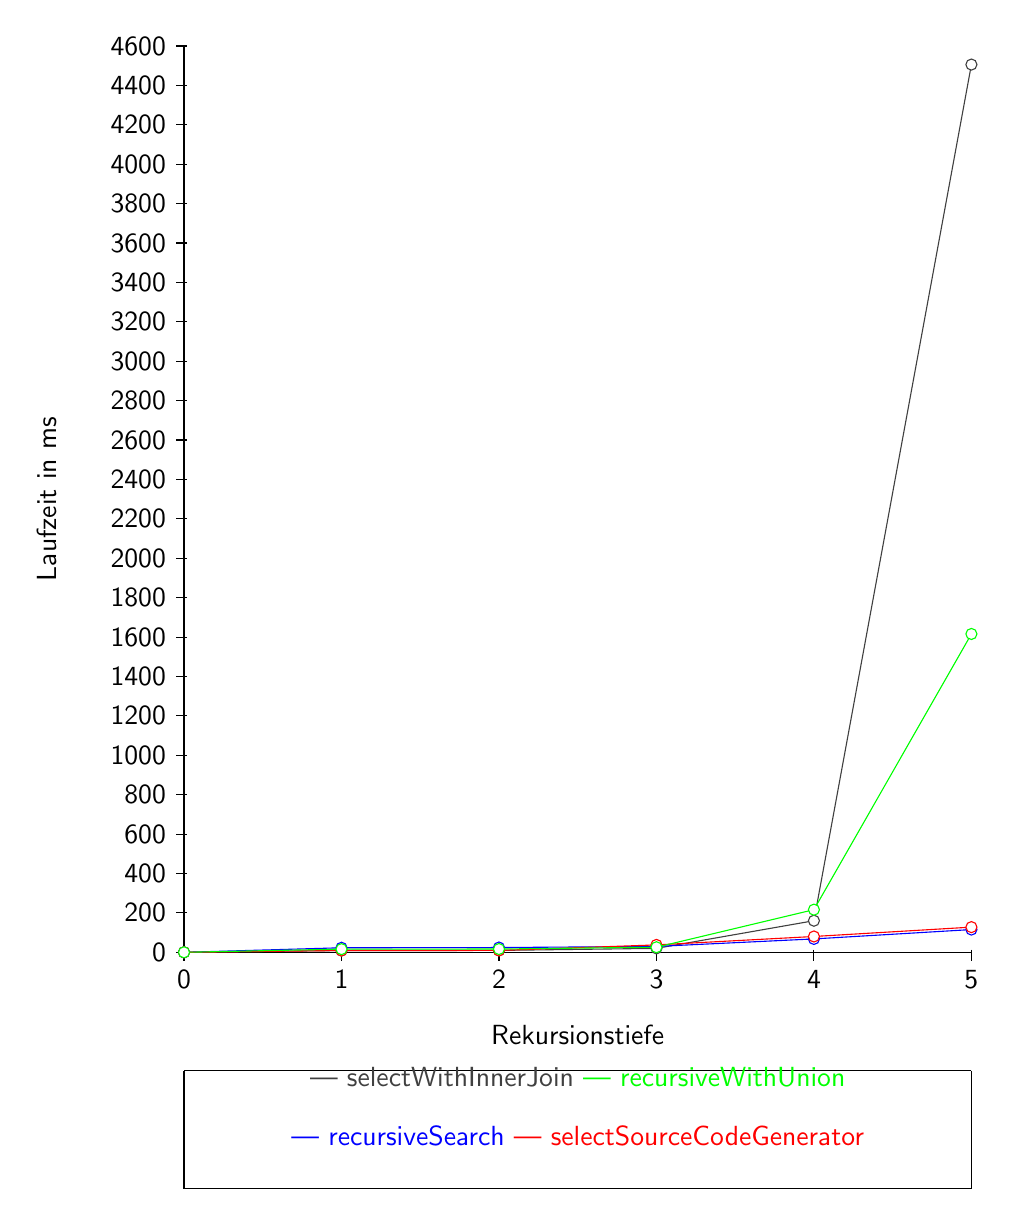
\begin{tikzpicture}[y=.0025cm, x=2cm,font=\sffamily]
	%axis
	\draw (0,0) -- coordinate (x axis mid) (5,0);
	\draw (0,0) -- coordinate (y axis mid) (0,4600);
	%ticks
	\foreach \x in {0,...,5}
	\draw (\x,1pt) -- (\x,-3pt)
	node[anchor=north] {\x};
	\foreach \y in {0,200,...,4600}
	\draw (1pt,\y) -- (-3pt,\y)
	node[anchor=east] {\y}; 
	%labels      
	\node[below=0.8cm] at (x axis mid) {Rekursionstiefe};
	\node[rotate=90, above=1.5cm] at (y axis mid) {Laufzeit in ms};
	%plots
	\draw[darkgray] plot[ mark=*, mark options={fill=white}] 
	coordinates{(0, 0)
		(1, 8.882)
		(2, 9.694)
		(3, 20.019)
		(4, 160.368)
		(5, 4505.545)
	};
	
	\draw[blue] plot[ mark=*, mark options={fill=white}] 
	coordinates{(0, 0)
		(1, 23.059)
		(2, 24.221)
		(3, 29.832)
		(4, 67.963)
		(5, 115.465)
	};
	\draw[red] plot[ mark=*, mark options={fill=white}] 
	coordinates{(0, 0)
		(1, 9.169)
		(2, 9.538)
		(3, 37.563)
		(4, 80.343)
		(5, 127.839)
	};
	\draw[green] plot[ mark=*, mark options={fill=white}] 
	coordinates{(0, 0)
		(1, 16.152)
		(2, 16.649)
		(3, 25.806)
		(4, 216.439)
		(5,1615.686)
	};
	
	\draw (0,-600) -- (5,-600) 
	(0,-600) -- (0,-1200)
	(0,-1200) -- (5,-1200)
	(5,-600) -- (5,-1200);
	\draw[draw=none] (0,0) -- (5,0) 
	node[draw=none, midway, yshift=-4.5em]
	{
		\textcolor{darkgray}{--- selectWithInnerJoin}
		\textcolor{green}{--- recursiveWithUnion} 
		
	};
	\draw[draw=none] (0,-600) -- (5,0) 
	node[draw=none, midway, yshift=-4.5em]
	{
		\textcolor{blue}{--- recursiveSearch} 
		\textcolor{red}{--- selectSourceCodeGenerator}
	};
	\end{tikzpicture}
	\caption{ public\_wiki\_vote}
\end{figure}

\begin{figure}[H]
	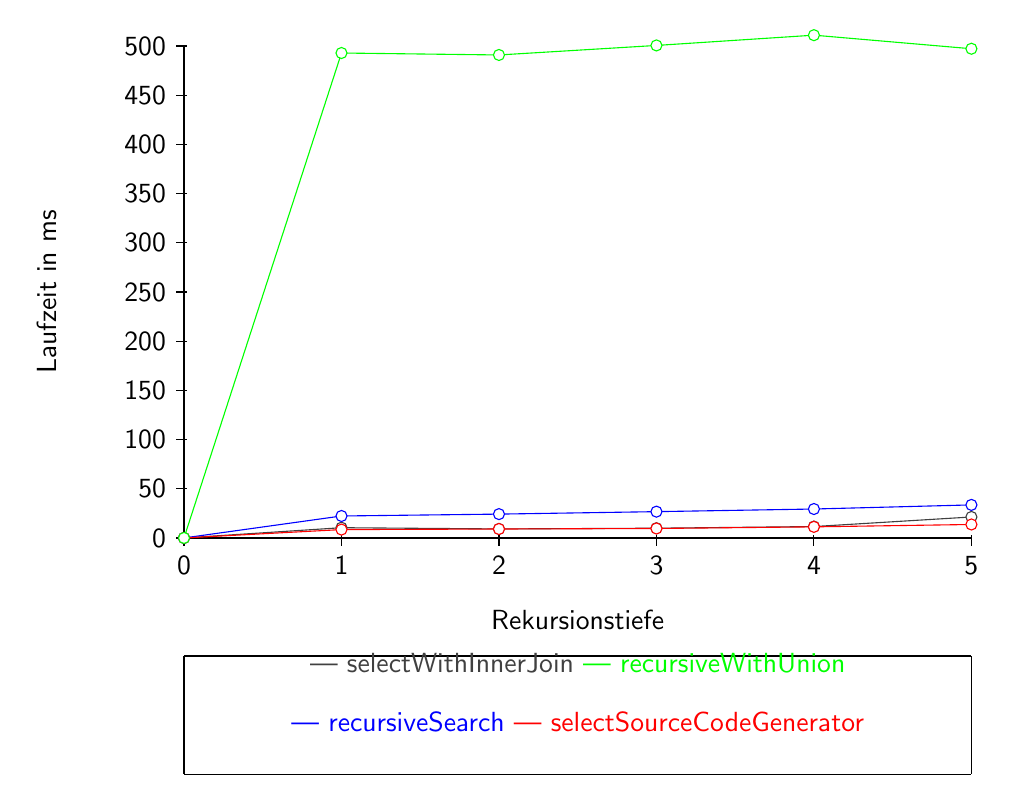
\begin{tikzpicture}[y=.0125cm, x=2cm,font=\sffamily]
	%axis
	\draw (0,0) -- coordinate (x axis mid) (5,0);
	\draw (0,0) -- coordinate (y axis mid) (0,500);
	%ticks
	\foreach \x in {0,...,5}
	\draw (\x,1pt) -- (\x,-3pt)
	node[anchor=north] {\x};
	\foreach \y in {0,50,...,500}
	\draw (1pt,\y) -- (-3pt,\y)
	node[anchor=east] {\y}; 
	%labels      
	\node[below=0.8cm] at (x axis mid) {Rekursionstiefe};
	\node[rotate=90, above=1.5cm] at (y axis mid) {Laufzeit in ms};
	%plots
	\draw[darkgray] plot[ mark=*, mark options={fill=white}] 
	coordinates{(0, 0)
		(1, 10.423)
		(2, 9.162)
		(3, 9.909)
		(4, 11.589)
		(5, 21.320)
	};
	
	\draw[blue] plot[ mark=*, mark options={fill=white}] 
	coordinates{(0, 0)
		(1, 22.322)
		(2, 24.235)
		(3, 26.731)
		(4, 29.409)
		(5, 33.586)
	};
	\draw[red] plot[ mark=*, mark options={fill=white}] 
	coordinates{(0, 0)
		(1, 8.505)
		(2, 9.090)
		(3, 9.629)
		(4, 11.286)
		(5, 13.694)
	};
	\draw[green] plot[ mark=*, mark options={fill=white}] 
	coordinates{(0, 0)
		(1, 492.834)
		(2, 490.843)
		(3, 500.531)
		(4, 510.964)
		(5, 497.172)
	};
	
	\draw (0,-120) -- (5,-120) 
	(0,-120) -- (0,-240)
	(0,-240) -- (5,-240)
	(5,-120) -- (5,-240);
	\draw[draw=none] (0,0) -- (5,0) 
	node[draw=none, midway, yshift=-4.5em]
	{
		\textcolor{darkgray}{--- selectWithInnerJoin}
		\textcolor{green}{--- recursiveWithUnion} 
		
	};
	\draw[draw=none] (0,-120) -- (5,0) 
	node[draw=none, midway, yshift=-4.5em]
	{
		\textcolor{blue}{--- recursiveSearch} 
		\textcolor{red}{--- selectSourceCodeGenerator}
	};
	\end{tikzpicture}
	\caption{ public\_youtube}
\end{figure}

\subsection{Standard SQL}

\subsection{Stored Procedures}
\subsection{PL/SQL-Recursion}
\subsection{Datenbankzugriffe}
\subsection{Zugriffsart Aggregation}
\subsection{Zugriffsart Traversierung}
\subsection{Interpretation der Ergebnisse}